% ==============================================================================
% TCC - Nome do Aluno
% Capítulo 3 - Projeto Arquitetural e Implementação
% ==============================================================================
\chapter{Algoritmos Dinâmicos}
\label{sec-dinamicos}

\section{Grafos Dinâmicos}
\label{sec-dinamicos-grafos}


\section{Algoritmo ARA*}
\label{sec-dinamicos-ara}

O algoritmo ARA* proposto em \citeonline{likhachev2008anytime}, está descrito nas listagens \ref{lst-dinamicos-ara-computepath}, \ref{lst-dinamicos-ara-key} e \ref{lst-dinamicos-ara-main}.

\begin{lstlisting}[mathescape, label=lst-dinamicos-ara-computepath, caption=Algoritmo ARA* - função de cálculo de caminho, float=htpb]
procedure ComputePath()
	while(key($s_{goal}$) > $min_{s \in OPEN(key(s))}$)
		remove s with smallest key(s) from OPEN;
		v(s) = g(s); CLOSED = CLOSED $\cup$ {s};
		for each successor s' of s
			if s' was never visited by ARA* before then
				v(s') = g(s') = $\infty$;
			if g(s') > g(s) + c(s, s')
				g(s') = g(s) + c(s, s');
				if s' $\notin$ CLOSED
					insert/update s' in OPEN with key(s');
				else
					insert s' into INCONS;
\end{lstlisting}

 
\begin{lstlisting}[mathescape, label=lst-dinamicos-ara-key, caption=Algoritmo ARA* - função da chave ordenadora da fila de prioridades, float=htpb]
procedure key(s)
	return g(s) + $\epsilon$ * h(s);
\end{lstlisting}

\begin{lstlisting}[mathescape, label=lst-dinamicos-ara-main, caption=Algoritmo ARA* - função principal, float=htpb]
procedure Main()
	g($s_{goal}$) = v($s_{goal}$) = $\infty$; v($s_{start}$) = $\infty$;
	g($s_{start}$) = 0; OPEN = CLOSED = INCONS = $\emptyset$;
	insert $s_{start}$ into OPEN with key($s_{start}$);
	ComputePath();
	publish current $\epsilon$-suboptimal solution;
	while $\epsilon > 1$
		decrease $\epsilon$;
		Move states from INCONS into OPEN
		Update the priorities for all s $\in$ OPEN according to key(s);
		CLOSED = $\emptyset$;
		ComputePath();
		publish current $\epsilon$-suboptimal solution;
\end{lstlisting}

Começando pela função principal (listagem \ref{lst-dinamicos-ara-main}), temos as variáveis g(s) e v(s) que correspondem ao valor da distância real calculada da origem $s_{start}$ até o vértice s (o valor de v(s), apesar de estar descrito no algoritmo conforme a literatura de origem, não é utilizado pelo algoritmo e por isso será ignorado na explicação que se segue). O valor de g($s_{goal}$) (distância real calculada da origem ao vértice destino) é atribuído como $\infty$ (infinito)\footnote{Vide nota de rodapé da seção \ref{sec-dijkstra-algoritmo}.}, enquanto que o valor de g($s_{start}$) é atribuído com o valor 0 (já que o valor da distancia real calculada se baseia a partir da origem). Em seguida são criados o conjunto "OPEN", "CLOSED" e "INCONS", correspondendo respectivamente ao conjunto dos "ABERTOS", "FECHADOS" e "INCONSISTENTES". Em seguida, $s_{start}$ é inserido na fila de prioridades do conjunto OPEN utilizado a função de chave ordenadora descrito na listagem \ref{lst-dinamicos-ara-key}, a qual utiliza a estratégia da heurística inflada (descrito a seguir).

A função de cálculo de caminho é então invocada pela função principal (listagem \ref{lst-dinamicos-ara-computepath}). Nesta função, o processo iterativo se faz enquanto o valor da chave de $s_{goal}$ for maior do que o valor da chave do termo mínimo da fila de prioridades. Enquanto isso for verdade, o vértice s, que corresponde ao valor do vértice com menor chave de OPEN, é removido deste e adicionado ao conjunto CLOSED. Para cada s', que representa o conjunto de vértices adjacentes de s, é verificado se tal vértice já foi visitado pelo algoritmo e em caso negativo, o seu valor de g(s') é atribuído como $\infty$ (infinito). Em seguida, é verificado se a distância calculada até o momento para s', g(s'), é maior do que a soma de g(s) mais o peso da aresta entre s e s'. Se caso positivo, g(s') é atribuído com esse novo valor. A seguir é verificado se o vértice s' não pertence ao conjunto dos fechados e em caso positivo, ele é adicionado/atualizado no conjunto OPEN baseando-se na função de chave ordenadora. Em caso contrário, ele é adicionado ao conjunto dos INCONS.

Após o cálculo do caminho e continuando a função principal (listagem \ref{lst-dinamicos-ara-main}), a solução $\epsilon$ sub-ótima é apresentada pelo algoritmo. A partir daí começa o processo iterativo em que o valor de $\epsilon$ é verificado se é maior do que 1. Em caso positivo, o valor de $\epsilon$ é decrescido por um fator de corte estipulado pelo programador. Os vértices pertencentes a INCONS são movidos para OPEN. E todas as chaves da fila de prioridades são atualizados considerando o novo valor de $\epsilon$. O conjunto CLOSED é limpo e a função de cálculo de caminho é invocada novamente, e  o resultado publicado.

\subsection{Heurística inflada e considerações sobre o algoritmo}
\label{sec-dinamicos-ad-consideracoes}

A principal diferença entre o algoritmo ARA* e o A* está na utilização da estratégia da heurística inflada. Ela consiste em utilizar a mesma função de ordenação de chaves da fila de prioridades do algoritmo A*, com a exceção de que o valor heurístico é multiplicado por um fator $\epsilon$. Isso faz com que menos vértices sejam visitados, já que os menos "promissores" serão jogados mais para o final da fila de prioridades enquanto que os mais "promissores" serão jogados para frente. Entretanto, ao se utilizar esta técnica perdemos a garantia do resultado ótimo do algoritmo (algo semelhante ao que ocorre quando não utilizamos heurísticas não-admissíveis. Vide subseção \ref{sec-aestrela-algoritmo-heuristica}).

Porém, "Uma grande vantagem de se utilizar a estratégia apresentada é que temos um limite superior para a solução encontrada. Suponha que a melhor solução tenha custo C*. Se utilizarmos uma busca com o A* com um valor real $\epsilon \geq 1$ multiplicando o valor heurístico na função de avaliação, então há a garantia que para a nova solução C, C* $\leq$ C $\leq \epsilon$ x C*. Portanto, se $\epsilon$ = 1, a solução encontrada é ótima." (Citar referência A).

Portanto a ideia principal é achar uma solução rápida, porém não-garantidamente ótima, atribuindo um valor $\epsilon$ maior do que 1, e a mediada que mais tempo é nos dado, diminuímos o valor de $\epsilon$ até termos $\epsilon$ = 1, em que a solução será garantidamente ótima. 

Outra estratégia utilizada é que para ganhar tempo, a cada novo valor de $\epsilon$ em que a função para cálculo de caminho é invocada (listagem \ref{lst-dinamicos-ara-computepath}), não é necessário recalcular todos os vértices visitados anteriormente, já que os mesmo permanecem na lista de abertos (tendo apenas suas chaves atualizadas com o novo valor de $\epsilon$ e consequentemente a ordem dos vértices também é reconfigurada de acordo com esses novos valores). Além disso, para caso haja um melhor caminho encontrado para um vértice que pertence aos fechados, este é enviando para os INCONS dos quais serão enviados para OPEN para serem recalculados na próxima iteração.

A figura \ref{fig-ara-exemplo}, contida em \citeonline{likhachev2008anytime}, mostra a aplicação da estratégia dita anteriormente.

\begin{figure}[H]
\centering
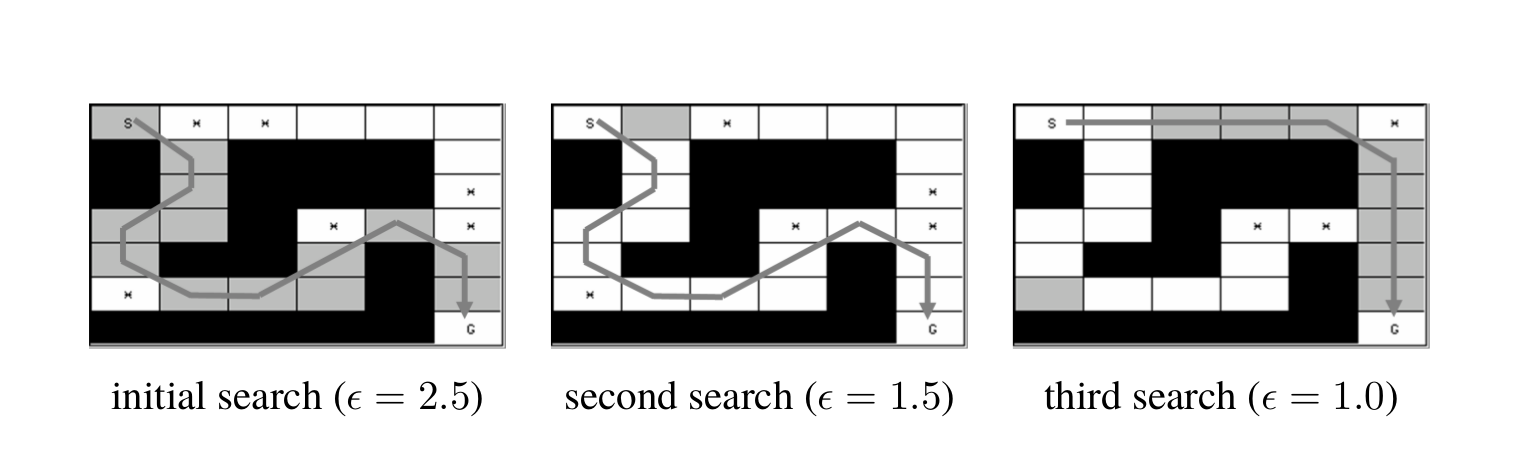
\includegraphics[width=.80\textwidth]{figuras/ara-3} 
\caption{Exemplo de aplicação da estratégia de diminuição do valor de $\epsilon$.}
\label{fig-ara-exemplo}
\end{figure}
\section{Algoritmo AD*}
\label{sec-dinamicos-ad}

O algoritmo AD* também proposto em \citeonline{likhachev2008anytime}, está descrito nas listagens \ref{lst-dinamicos-ad-set}, \ref{lst-dinamicos-ad-computepath}, \ref{lst-dinamicos-ad-key} e \ref{lst-dinamicos-ad-main}.

\begin{lstlisting}[mathescape, label=lst-dinamicos-ad-set, caption=Algoritmo AD* - função para determinar o conjunto ao qual vértice pertencerá, float=htpb]
procedure UpdateSetMembership(s)
	if ($v(s) \neq g(s)$)
		if (s $\notin$ CLOSED) insert/update s in OPEN with key(s);
		else if (s $\notin$ INCONS) insert s in INCONS;
	else
		if (s $\in$ OPEN) remove s from OPEN;
		else if (s $\in$ INCONS) remove s from INCONS;
\end{lstlisting}

\begin{lstlisting}[mathescape, label=lst-dinamicos-ad-computepath, caption=Algoritmo AD* - função de cálculo de caminho, float=htpb]
procedure ComputePath()
	while(key($s_{goal}$) > $min_{s \in OPEN(key(s))}$ OR v($s_{goal}$) < g($s_{goal}$)) 
		remove s with smallest key(s) from OPEN;
		if v(s) > g(s)
			v(s) = g(s); CLOSED = CLOSED $\cup$ {s};
			for each successor s' of s
				if s' was never visited by AD* before then
					v(s') = g(s') = $\infty$;bp(s') = null;
				if g(s') > g(s) + c(s, s')
					g(s') = g(s) + c(s, s');
					bp(s') = s;
					g(s') = g(bp(s')) + c(bp(s'),s'); UpdateSetMembership(s');
		else
			v(s) = $\infty$; UpdateSetMembership(s);
			for each successor s' of s
			if s' was never visited by AD* before then
				v(s') = g(s') = $\infty$;bp(s') = null;
			if bp(s') = s
				bp(s') = $argmin_{s'' \in pred(s')}$ v(s'') + c(s'',s');
				g(s') = v(bp(s')) + c(bp(s'),s'); UpdateSetMembership(s');
\end{lstlisting}

\begin{lstlisting}[mathescape, label=lst-dinamicos-ad-key, caption=Algoritmo AD* - função da chave ordenadora da fila de prioridades, float=htpb]
procedure key(s)
	if (v(s) $\geq$ g(s))
		return [g(s) + $\epsilon$ * h(s); g(s)];
	else
		return [v(s) + h(s); v(s)];
\end{lstlisting}

\begin{lstlisting}[mathescape, label=lst-dinamicos-ad-main, caption=Algoritmo AD* - função principal, float=htpb]
procedure Main()
	g($s_{goal}$) = v($s_{goal}$) = $\infty$; v($s_{start}$) = $\infty$;bp($s_{goal}$) = bp($s_{start}$) = null;
	g($s_{start}$) = 0; OPEN = CLOSED = INCONS = $\emptyset$; $\epsilon = \epsilon_{0}$;
	insert $s_{start}$ into OPEN with key($s_{start}$);
	forever
		ComputePath();
		publish current $\epsilon$-suboptimal solution;
		if $\epsilon = 1$
			wait changes in edge costs;
		for all directed edges (u,v) with changed edge costs
			update the edge cost c(u,v);
			if ( $v \neq s_{start}$ AND v was visited by AD* before)
				bp(v) = $argmin_{s'' \in pred(v)}$ v(s'') + c(s'',v);
				g(v) = v(bp(v)) + c(bp(v),v); UpdateSetMembership(v);
		if significant edge cost changes were observed
			increase $\epsilon$ or re-plan from scratch (i.e., re-excute Main function);
		else if $\epsilon > 1$
			decrease $\epsilon$;
		Move states from INCONS into OPEN
		Update the priorities for all s $\in$ OPEN according to key(s);
		CLOSED = $\emptyset$;
\end{lstlisting}

O algoritmo é muito semelhante em sua execução ao ARA*, já que o AD* é uma adaptação do mesmo. A função principal (listagem \ref{lst-dinamicos-ad-main}) começa iniciando os valores de g($s_{goal}$), v($s_{goal}$) e v($s_{start}$) como $\infty$, bp($s_{start}$) como nulo e g($s_{start}$) como 0. Em seguida o vértice $s_{start}$ é inserido na fila de prioridades de acordo com  a função de chave ordenadora descrita na listagem \ref{lst-dinamicos-ad-key}. Disso, é invocado a função de cálculo de caminho (listagem \ref{lst-dinamicos-ad-computepath}).

Essa função trabalha da seguinte forma: inicialmente se verifica se o valor da chave de $s_{goal}$ é maior do que a menor chave da fila de prioridades (condição semelhante ao do algoritmo ARA*, vide listagem \ref{lst-dinamicos-ara-computepath}) ou se o valor de v($s_{goal}$) é menor do que o valor de g( $s_{goal}$ ). Se caso for verdade, o processo iterativo é inciado. O vértice s, que corresponde ao vértice com menor chave na fila de prioridades é removido do conjunto OPEN, e é verificado se o valor de v(s) é maior do que o g(s) (ou seja, se o valor da distância calculada da busca anterior é maior do que o valor da busca atual, esse é o caso normal do algoritmo). Sendo verdade, o algoritmo segue a mesma forma de execução do ARA*, conforme descrito na seção \ref{sec-dinamicos-ara}. A diferença de tratamento ocorre quando a condição inicial não ocorre, e neste caso, o valor de v( s ) é atribuído como $\infty$, e para cada vértice s' de s é verificado se este já havia sido visitado pelo algoritmo. Se caso não havia sido visitado, os valores de v( s' ), g( s' ) são inciados como $\infty$ e bp( s') é inciado como nulo. Seguindo, é verificado se o bp( s' ) é igual o vértice s. Se caso sim, o bp( s' ) é atualizado com o vértice predecessor de s', s'', cuja a função v(s'') + c( s'', s') é a menor. Feito isso, o valor de g( s' ) é atualizado com esse novo valor. Em seguida a função de determinação para qual conjunto pertencerá s' é chamado (função "UpdateSetMembership").

A função de determinação ao qual conjunto pertencerá funciona de uma maneira muito simples. Caso os valores de v( s ) e g( s ) sejam diferentes, a função é igual ao que ocorre no processo de atribuição de conjunto do ARA* (vide listagem \ref{lst-dinamicos-ara-computepath}), a diferença ocorre quando esses valores são iguais (ou seja, não houve mudança de valores entre a busca atual e a anterior), o vértice é removido de OPEN caso esteja nele ou removido de INCONS caso pertença a este. Isso feito para que este vértice não precise ser calculada nesta busca ou na próxima (caso esteja em INCOS).

Voltando ao método principal (listagem \ref{lst-dinamicos-ad-main}), a função segue o mesmo padrão da ARA*, a única exceção se dá quando mudanças no grafo são detectadas (mudança dos pesos das arestas). Neste caso, para cada aresta (u,v) mudada, é atribuído ao valor bp( v ), o vértice s'', predecessor de v, cuja a função v( s'' ) + c( s'', v) seja mínima. Consequentemente, o valor de g( v ) é atualizado conforme esse valor e a função de atribuição de conjunto é invocada. 